\lecture{13}{9 aprile 2024}

\section{Onde sferiche}
Spesso può essere utile cambiare rappresentazione del problema per coglierne la simmetria. Ad esempio, un'onda che parte da un punto e si sviluppa nello spazio tridimensionale sarà simmetrica rispetto all'origine. Vicino alla sorgente la rappresentazione di onda piana non va più bene. Proviamo con le coordinate polari sferiche:
\begin{equation}
	\begin{cases}
		x = r \sin\theta \cos\varphi \\
		y = r \sin \theta \sin \varphi \\
		z = r \cos \theta 
	\end{cases}
\end{equation}
I versori sono convenzionalmente diretti nel verso in cui varia il versore aumentando la coordinata di riferimento (ad esempio: il versore \(\vec{\hat{e}_\theta}\) ha sempre componente \(z\) negativa, perché aumentare \(\theta \) porta il punto "in giù".).
In coordinate sferiche dobbiamo tenere conto di come varia il laplaciano:
\begin{equation}
	\laplacian{} = \frac{1}{r^{2} } \frac{\partial }{\partial r} \left( r^{2} \frac{\partial }{\partial r}  \right)
	+ \frac{1}{r^{2} }\left( \frac{1}{\sin \theta } \frac{\partial }{\partial \theta } \left( \sin \theta \frac{\partial }{\partial \theta} \right) + \frac{1}{\sin ^{2} \theta } \frac{\partial ^{2} }{\partial \varphi ^{2} }   \right)     
\end{equation}
Questo risultato si può ottenere facilmente con i coefficienti di Lamè.
Di conseguenza si può riscrivere l'equazione di D'Alembert con le nuove coordinate:
\begin{equation}
	\laplacian{\xi (r,\theta ,\varphi ,t)}=\frac{1}{v^{2} }	\frac{\partial ^{2} \xi (r,\theta ,\varphi ,t)}{\partial t^{2} }  
\end{equation}
\subsection{Soluzione delle onde sferiche}
Si può mostrare che esistono soluzioni generiche di questo tipo:
\begin{equation}
	\xi (\vec{r},t)=\xi (r,\theta ,\varphi ,t)=\frac{f(r\mp vt)}{r}Y^m_l(\theta ,\varphi )
\end{equation}
\(\forall f \in \mathcal{C} ^{2}\) e per particolari funzioni \(Y_l^m \in \mathcal{C} ^{2} \) infinite ma numerabili, gli indici sono \(l=0,1,\dots , \infty ;\ m =-l, \dots ,0,\dots +l\) (WOW! In futuro rappresenteranno gli orbitali). Queste funzioni soddisfano equazioni del tipo:
\begin{figure}[H]
	\centering
	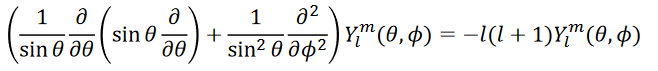
\includegraphics[width=0.6\textwidth]{screenshots/2024-04-09-11-38-55.png}
\end{figure}
Le \(Y_l^m\) sono dette \emph{armoniche sferiche}.
\begin{figure}[H]
	\centering
	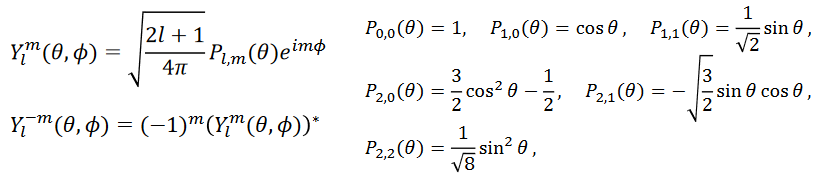
\includegraphics[width=0.7\textwidth]{screenshots/2024-04-09-11-41-43.png}
\end{figure}
Noi generalmente guarderemo le armoniche sferiche con \(l=0,1\). Le funzioni sono ortonormali sulla superficie della sfera (nello spazio delle funzioni definite su \((\theta ,\varphi )\)).
Guardiamo ora i casi che si possono presentare per il termine dipendente da \(r\mp vt\).
\begin{itemize}
	\item \(\frac{f(r-vt)}{r}\) rappresenta un'onda sferica uscente dall'origine;
	\item \(\frac{f(r+vt)}{r}\) rappresenta un'onda sferica che va verso l'origine.
\end{itemize}
Dimostriamo che \(\xi (r,\theta ,\varphi ,t) = \frac{f(r-vt)}{r}\) è una soluzione dell'equazione di D'Alembert (abbiamo scelto \(Y_0^0(\theta ,\varphi )=\sqrt{\frac{1}{4\pi }} \)):
\begin{figure}[H]
	\centering
	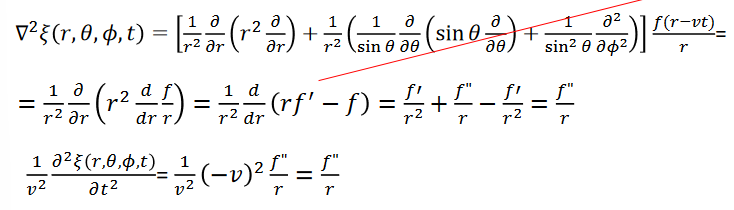
\includegraphics[width=0.6\textwidth]{screenshots/2024-04-09-11-47-14.png}
\end{figure}
Le onde sferiche con \(f(r-vt)=A\cos (kr-\omega t +\alpha )\) sono dette \emph{onde armoniche sferiche}:
\begin{equation}
	\xi (r,\theta ,\varphi ,t)=\frac{A}{r}\cos (kr- \omega t+\alpha )Y_m^l(\theta ,\varphi )
\end{equation}
Si nota che le onde sferiche possono avere una periodicità temporale (nel caso di onde armoniche ce l'hanno, in altri casi potrebbero non averla!) con periodo \(T_p=\frac{2\pi }{\omega }\), ma non c'è periodicità spaziale per la presenza del fattore \(\quotient{1}{r}\). Questa può essere tuttavia chiamata "pseudo-periodicità" spaziale con lunghezza d'onda \(\lambda =\quotient{2\pi }{k} \).

\paragraph{Significato fisico del fattore \(\quotient{1}{r} \)}
Il fattore \(\quotient{1}{r} \) è finora solo un fatto matematico, tuttavia si può comprendere il suo significato fisico attraverso l'energia.
\begin{note}
	Ricorda che valeva:
	\begin{figure}[H]
		\centering
		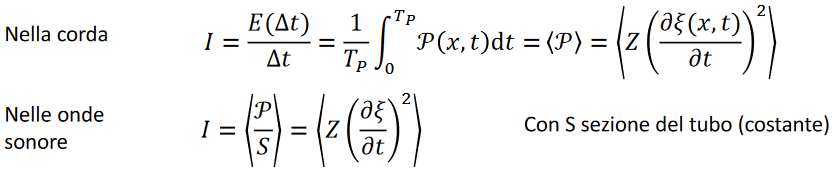
\includegraphics[width=0.7\textwidth]{screenshots/2024-04-09-11-57-41.png}
	\end{figure}
	Per le onde armoniche era \(I=\frac{1}{2}Z \omega ^{2} A^{2} \).
\end{note}
Nel caso di onde sferiche la potenza a distanza \(r\) si distribuisce su un'area pari a \(S=4\pi r^{2} \). Quindi
\begin{equation}
	I = \left\langle \frac{\mathcal{P} }{S} \right\rangle = r^{-2} \frac{1}{2}Z \omega ^{2} A^{2} 
\end{equation}
L'impedenza non può calare come \(r^{-2}\), la pulsazione neanche. Quindi dobbiamo concludere che \(A=\quotient{A^{\prime} }{r} \), ossia:
\begin{figure}[H]
	\centering
	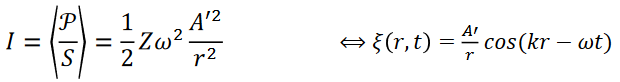
\includegraphics[width=0.6\textwidth]{screenshots/2024-04-09-12-03-46.png}
\end{figure}